\chapter{Comparison of Architectures and Loss Functions}
\label{chap:architecture}
Different architectures of DNNs means different combinations of layers. In this chapter, all of the architectures I'm going to talk about is based on a general model for sound type classification. On the basis of this general model, replacement of some of the layers produce different architectures. The replaced layers are mainly loss layers, which also effects the optimization during training. In this chapter, I will compare 3 types of architectures and discuss the experiment results.

\section{Methods}
The experiments are all carried out on NI(Neural Information Processing Group of TU Berlin) computing servers. In order to accelerate the training process, GPU mode is prefered as the solver\_mode. 

The performance metric is sensitivity, specificity and balanced accuracy.%TODO:\ref{chapter1 equation}
For a classifier, which classifies all the test sources as positive, it still get a $100\%$ sensitivity. If the amount of true positive points is equal to the amount of true negative points, the accuracy can still reach $50\%$. Considering only the accuracy, the classifier tends to make positive or negative decisions w.r.t the prior of positive and negative sources. That's why  sensitivity, specificity and balanced accuracy were chosen as the performance metrics. Caffe didn't implement a layer for the calculation of sensitivity and specificity. Accuracy layer produces a metric which can't describe the performance of a classifier well. In order to calculate the sensitivity, I used python interface in Caffe to extract intermediate outputs of the DNN from the '.caffemodel' files and calculate these three performance metrics to complete the comparison of different DNN architecture. There are in total 11 classes of sound types, so the performance metrics were calculated for each of these sound types. 

\subsection{Architectures and Loss Functions}
%Motivations(why use these different Archs->because of the label representation as 0-1 vector)\\
%One-Against-All
%def.,motivation,result\\
%SoftmaxWithLoss
%def.,motivation,result\\
%SigmoidCrossEntropy
%def.,motivation,result,also the experiment with only 'ratemap' features
\subsubsection{One-Against-All Model}
Sound type classification can be seen as a multi-class classification problem. If we don't consider multi-label classification, a simple model which gives out one scalar output that indicates the class label can be easily constructed in DNN. This model is called one-against-all model in this thesis. This model trains a classifier for 12 classes(11 named classes and a general 'anything else' class). The main part of One-against-All architecture consists of 2 convolutional layers, 1 pooling layer, 2 innerproduct layers, 3 ReLU layers, a dropout layer and a loss layer. The visualization of this model is shown in Fig.\ref{fig:one-vs-all}

\begin{figure}[h!]
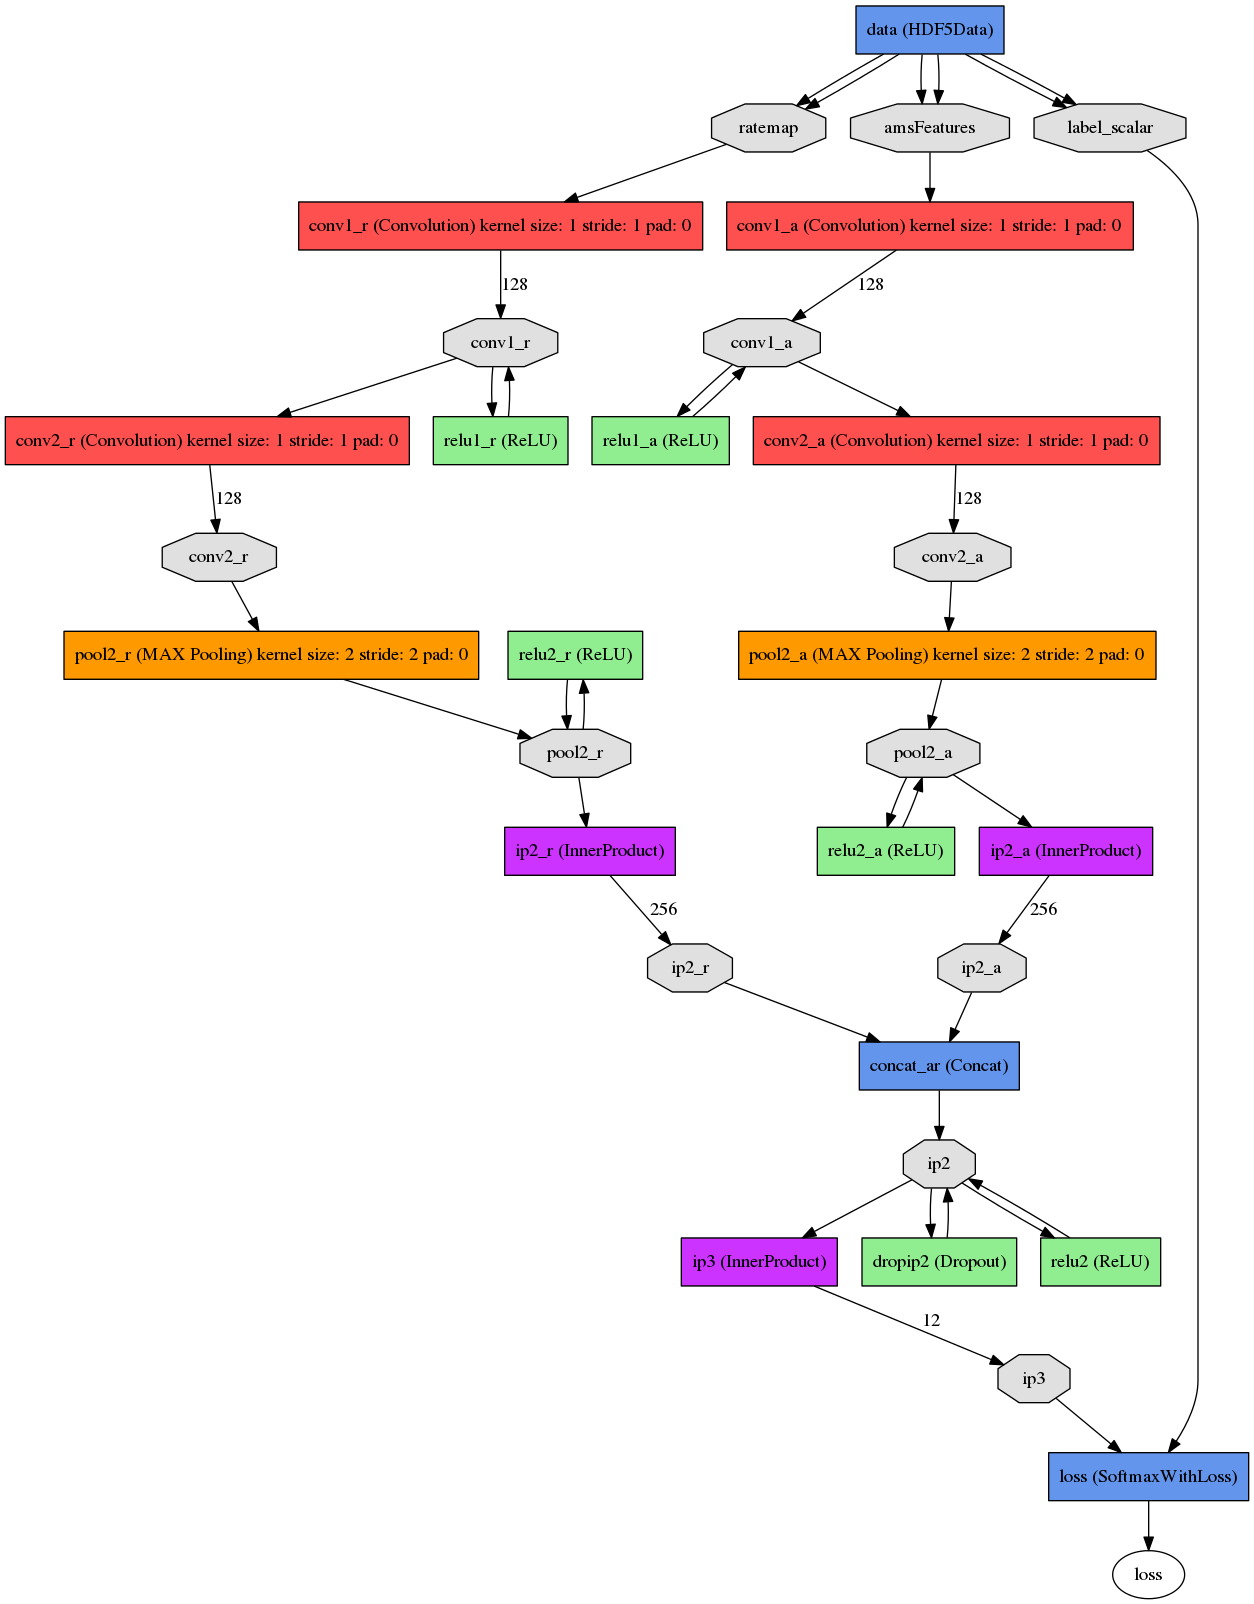
\includegraphics[scale=0.33]{../image/chapter2/one-vs-all.png}
\caption{One-Against-All Model architecture visualization}
\label{fig:one-vs-all}
\end{figure}
Convolutional layers produce intermediate feature images. As discussed in previous chapter. The adoption of convolutional layers helps in decreasing the weights, which has a positive influence in preventing overfitting problem. 
 
Pooling layers can be seen as a downsampling operation. The input features are convoluted with simple filters, which is usually of size $3\times3$. Pooling layers reduce the amount of parameters and computation in the network, and hence also control the overfitting problem. 
 
ReLU layer implements the activation function, defined as:
\begin{align}
f(x) = max(0,x)
\end{align}
In deep neural networks, back propagation through multiple  multiple layers with sigmoid activation function may cause the gradient vanish. Compared with sigmoid activation function, ReLU has a constant gradient, as a result, it can be used to reduce likelihood of vanishing gradient. That's why ReLU layers are used in our DNN model.

Dropout layers randomly switch off the updating of part of weights in the network during training process. As a result, drop layers also help to control overfitting.  The percentage of dropped weights can be defined as a parameter in dropout layer definition in Caffe. In this thesis, this parameter was set to $0.5$.

The loss layer used in One-Against-All model is 'SoftmaxWithloss' layer. The softmax loss layer computes the multinomial logistic loss of the softmax of its input scores. It takes a batch size of score vectors and true label vectors as inputs. The input scores from previous Innerproduct layer indicates the probability of the assignment to one class label, in other words, the output decided label would be the index with largest score value in the score vector.
\begin{align}
	\hat{p}_{nk}&=exp(x_{nk})/[\Sigma_{k'}exp(x_{nk'})]\\
	E &= -\frac{1}{N}\Sigma_{n=1}^{N}log(\hat{p}_{nl_n})
\end{align}
Where $\hat{p}_{nk}$ means the probability of input source indexed as $n$ to be classified as class $k$.\\
$x_{nk}$ is the input score of the loss layer. $n$ indicates the input source, $k$ is the index of the score vector from previous layer. The score vector is a 12-dimensional including the score for 'anything else' class.\\
$E$ is the computed cross-entropy classification loss. $l_n$ is the target label of input source indexed as $n$.
\subsubsection{SoftmaxWithLoss Model}
If we consider to build 11 binary classifiers using DNN, based on the idea of Lasso binary classifier, the new model can produce a label vector. As a result, this new DNN model can also do the multi-label classification. In this thesis we call this new model SoftmaxWithLoss model.

The basic architecture of the SoftmaxWithLoss model is almost the same as the One-Against-All model. In order to construct a classifier bank inside this network, some changes on the layer that outputs the score vectors should be made. In One-Against-All model, the scores come from an Innerproduct layer, and were passed directly to SoftmaxWithLoss Layer, which calculate an overall loss value as the object function for back propagation. In this SoftmaxWithLoss Model, instead of constructing a 12-dimensional score vector, the output from previous Innerproduct layer, which is in this case a 256-dimensional vector, are further send to 11 independent Innerproduct layers, the new scores become 2-dimensional vectors and go to 11 independent SoftmaxWithloss layers. The connection between these Innerproduct layers and SoftmaxWithloss layers are one-to-one. At this point, the network was splitted into 11 branches to train 11 binary classifiers. In each iteration of the model optimization, the model takes a batch size of input sources and split the true labels of the sources into 11 groups w.r.t the label values. The split of true labels are carried out by one Slice layer. These 11 groups of true labels are then passed to these 11 SoftmaxWithLoss layers separately. During the back propagation, the parameters of these Innerproduct layers will be trained to achieve 11 binary classification tasks. Fig.\ref{fig:slicing} shows how this branching works. 
\begin{figure}[h!]
	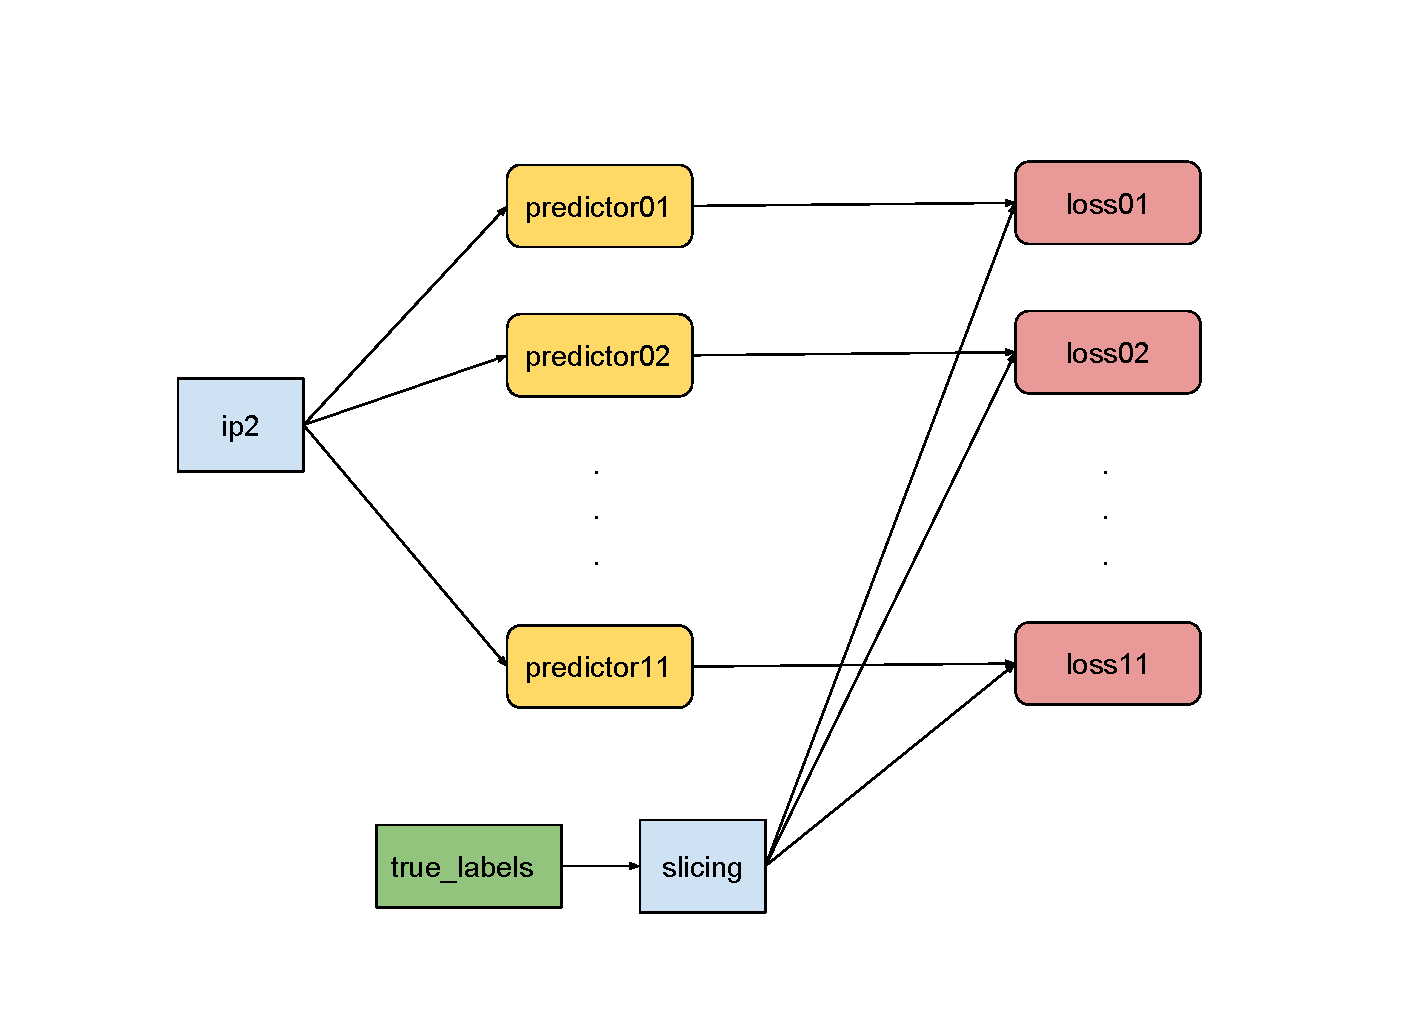
\includegraphics[scale=0.5]{../image/chapter2/slicing.pdf}
	\label{fig:slicing}
	\caption{Split of the labels for 11 binary classifier training}
\end{figure}
\subsubsection{SigmoidCrossEntropy Model}
The application of SoftmaxWithLoss layer makes the classification decision in a probabilistic way. If we want to use it for multi-label classification, the only way is to construct a bank of binary classifiers as the SoftmaxWithLoss model. If we consider another decision policy, that sets threshold for the scores and gives out a binary label vector, this also solves the multi-label classification problem. Sigmoid function can maps the scores to probability prediction vectors, each of which only answer the yes-or-no question w.r.t a decided threshold. Inspired by this idea, the SigmoidCrossEntropy Model is constructed using SigmoidCrossEntropy as the loss function. 
\begin{align}
\hat{p}_n &=\sigma(x_n) \\
E = -1\frac{1}{n}\Sigma_{n=1}^{N}[y_nlog\hat{p}_n+(1-y_n)log(1-\hat{p}_n)]
\end{align}
Where $\hat{p}_{n}$ is the mapped probability from score $x_n$.\\
$y_n$ is the target label of source index as $n$.
$E$ is the computed cross-entropy classification loss. 
\subsection{Implementation Details}
Due to the complexity of DNN models, the training process requires usually 100000 iterations to converge. The optimization method used in this chapter is Stochastic Gradient Descent(SGD). The general solver protocol settings are listed in Tab.\ref{tab:solversetting}
\begin{table}[h!]
	\begin{tabular}{|c|c|c|c|c|c|c|}
		\hline base\_lr & lr\_policy & gamma & stepsize & momentum & weight\_decay & solver\_mode \\ 
		\hline 1e-4 & step & 0.1 & 30000 & 0.99 & 0.0005  & GPU \\ 
		\hline 
	\end{tabular} 
	\label{tab:solversetting}
	\caption{Optimization Solver Settings}
\end{table}
I also experimented a bit with the Dropout Layer. For each of these three models, I carried out 2 expriments, one with dropout layer, the other without. The dropout ratio were all set to $0.5$.
%(Implementations details enable readers to recover the implementation)\\
%discuss about parameters
\section{Results and Discussion}
\subsection{Learning Curve}
%Also compare with Lasso results
Fig.\ref{fig:learningcurve} shows the learning curve of three models. In each  diagram, the solid lines represent for the results of the model with a dropout layer while the dash line without dropout layer.
For One-Against-All model and SigmoidCrossEntropy model the difference of the performances seems not so obvious. While in SoftmaxWithLoss model, the adoption of dropout layer contributes a lot for the good performance.
All of these three models get quite high specificity while quite low sensitivity. This means these three models tend to make negative decision. In the rest of this thesis, the main task is to tackle this problem, in order to find a better model with satisfying sensitivity. 
\begin{figure}
\subfloat[\label{subfig-1:1-vs-all}]{%
	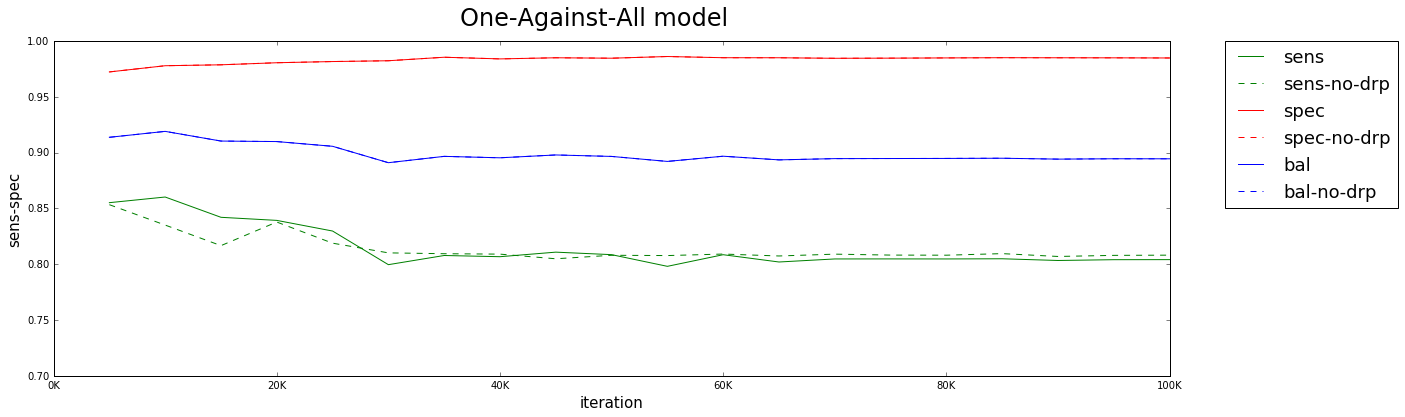
\includegraphics[scale=0.3]{../image/chapter2/one-against-all.png}
}
\hfill
\subfloat[\label{subfig-2:sft}]{%
	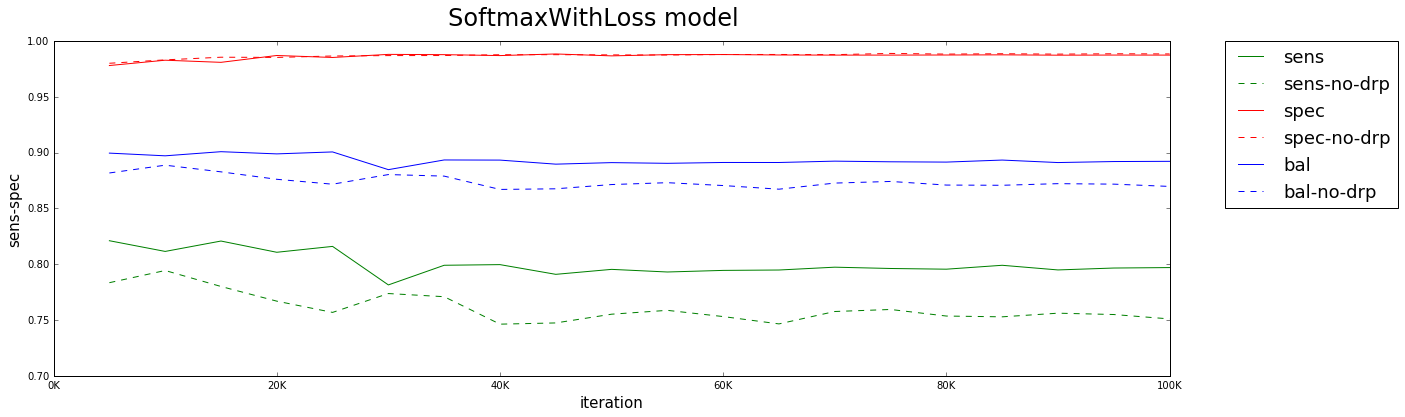
\includegraphics[scale=0.3]{../image/chapter2/SoftmaxWithLoss.png}
}
\hfill
\subfloat[\label{subfig-3:sce}]{%
	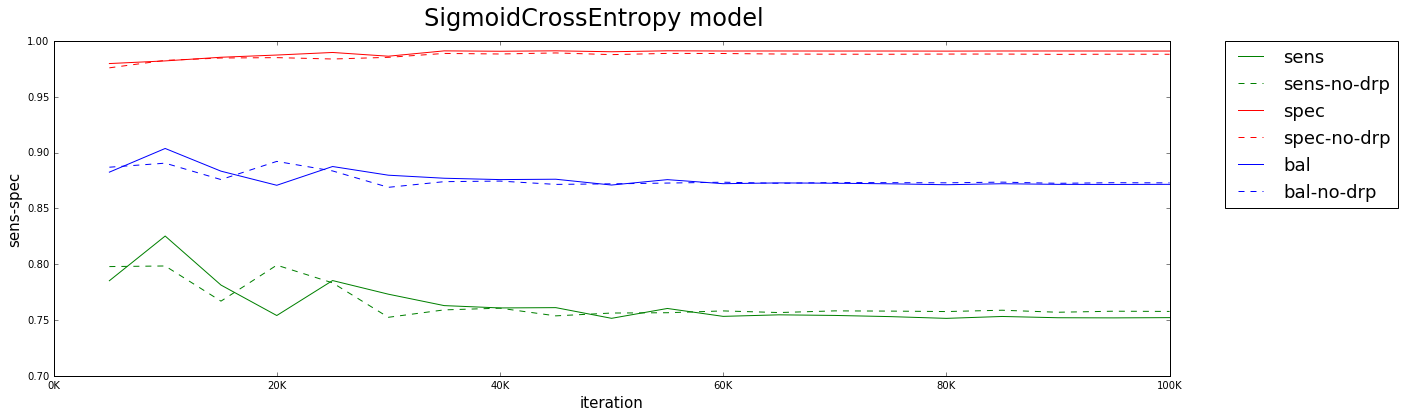
\includegraphics[scale=0.3]{../image/chapter2/SigmoidCrossEntropy.png}
}
\caption{Learning curve of 3 architectures}
\label{fig:learningcurve}
\end{figure}
\subsection{Comparison of Three Architectures}
Tab.\ref{tab:spec} shows the specificity accuracy metric for these three architectures. As mentioned above, there's no much difference when comparing these three models with sensitivity metric. However it shows much difference when focusing on the sensitivity metric. As shown in Tab.\ref{tab:sens}, the One-Against-All model shows a pretty good performance. It seems that SigmoidCrossEntropy model doesn't perform well. Considering the decision policy, SigmoidCrossEntropy model requires a proper setting of threshold. To see how well SigmoidCrossEntropy model can perform, I also plotted the Receiver Operating Characteristic(ROC) curve, see Fig.\ref{fig:rocSCE}. When classifying test sources from type 'alarm', 'crash' and 'engine', the performance has more critical limits than the others. For the other 8 sound types, SigmoidCrossEntropy can still get a good performance if the threshold is properly set. From the sensitivity table Tab.\ref{tab:sens}, 'phone' and 'piano' are also considered as sound types that are difficult to make a classification decision for SoftmaxWithLoss model and One-Against-All model. So in the rest of this thesis, I will focus on SigoidCrossentropy model and do some other improvement based on this model.

\begin{figure}[h!]
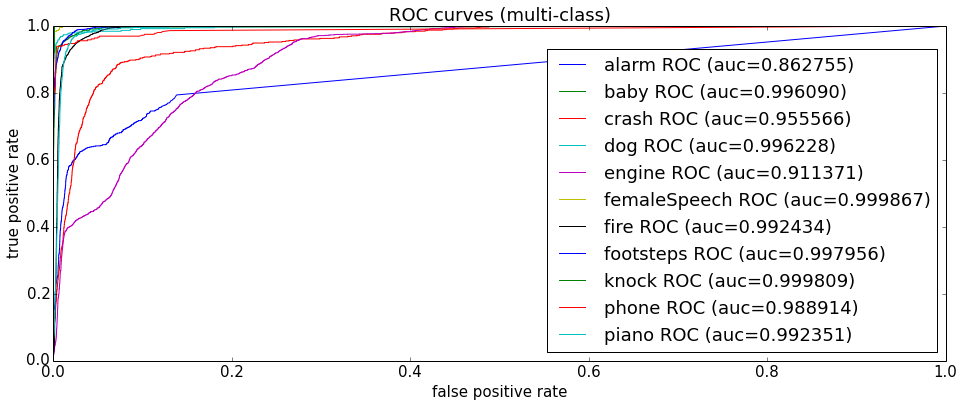
\includegraphics[scale=0.35]{../image/chapter2/rocSCE.png}
\label{fig:rocSCE}
\caption{ROC curve of SigmoidCrossEntropy model(with dropout layer)}
\end{figure}
\begin{table}[h!]
	\caption{Specificity of 3 models(with dropout layer)}
	\label{tab:spec}
	\begin{tabular}{|c|c|c|c|}
		\hline	model	&	\textbf{One-against-all}	&	\textbf{SoftmaxWithLoss}	&	\textbf{SimoidCrossEntropy}	\\
		\hline	alarm 	&	0.997286	&	0.993522	&	0.999168	\\
		\hline	baby 	&	0.981697	&	0.988665	&	0.991179	\\
		\hline	crash 	&	0.961532	&	0.975773	&	0.972213	\\
		\hline	dog 	&	0.996824	&	0.998712	&	0.99927	\\
		\hline	engine 	&	0.941389	&	0.946589	&	0.972967	\\
		\hline	femS 	&	0.999658	&	0.999658	&	0.999701	\\
		\hline	fire 	&	0.983448	&	0.976656	&	0.985964	\\
		\hline	ftStp 	&	0.987015	&	0.991237	&	0.989557	\\
		\hline	knock 	&	0.997626	&	0.99805	&	0.998813	\\
		\hline	phone 	&	0.995454	&	0.999571	&	0.999743	\\
		\hline	piano 	&	0.990786	&	0.992629	&	0.992497	\\
		\hline
	\end{tabular} 
\end{table}
\begin{table}[h!]
	\caption{Sensitivity of 3 models(with dropout layer)}
	\label{tab:sens}
	\begin{tabular}{|c|c|c|c|}
	\hline	model	&	\textbf{One-against-all}	&	\textbf{SoftmaxWithLoss}	&	\textbf{SimoidCrossEntropy}	\\
	\hline	alarm 	&	0.320958	&	0.585629	&	0.152096	\\
	\hline	baby 	&	0.95825	&	0.905567	&	0.942346	\\
	\hline	crash 	&	0.763889	&	0.71142	&	0.666667	\\
	\hline	dog 	&	0.937173	&	0.89267	&	0.876963	\\
	\hline	engine 	&	0.416096	&	0.406678	&	0.421233	\\
	\hline	femS 	&	0.962547	&	0.962547	&	0.940075	\\
	\hline	fire 	&	0.962135	&	0.94294	&	0.903234	\\
	\hline	ftStp 	&	0.982477	&	0.945015	&	0.947432	\\
	\hline	knock 	&	1	&	1	&	1	\\
	\hline	phone 	&	0.732782	&	0.738292	&	0.713499	\\
	\hline	piano 	&	0.808774	&	0.67604	&	0.709786	\\
	\hline
	\end{tabular} 
\end{table}

To check whether such bad performance comes from overfitting. I also carried out an experiment for SigmoidCrossEntropy model, where I replaced the test dataset with training dataset. The experiment result is shown in Tab.\ref{tab:SCEoverfitting}
\begin{table}[h!]
	\caption{SigmoidCrossEntropy model tested on training dataset}
	\label{tab:SCEoverfitting}
	\centering
	\begin{tabular}{|c|c|c|c|}
		\hline	class 	&	 \textbf{sensitivity}	&	 \textbf{specificity} 	&	 \textbf{bal\_acc}	\\
		\hline	alarm 	&	0.999742	&	0.999227	&	0.999484	\\
		\hline	baby 	&	1	&	0.99928	&	0.99964	\\
		\hline	crash 	&	0.996755	&	0.998332	&	0.997544	\\
		\hline	dog 	&	1	&	0.999828	&	0.999914	\\
		\hline	engine 	&	0.982397	&	0.997431	&	0.989914	\\
		\hline	femS 	&	1	&	0.999966	&	0.999983	\\
		\hline	fire 	&	0.984352	&	0.998883	&	0.991617	\\
		\hline	footS 	&	0.9971	&	0.999394	&	0.998247	\\
		\hline	knock 	&	1	&	0.999953	&	0.999977	\\
		\hline	phone 	&	1	&	0.999937	&	0.999969	\\
		\hline	piano 	&	0.999139	&	0.999567	&	0.999353	\\
		\hline
	\end{tabular} 
\end{table}
When testing on the training dataset, SigmoidCrossEntropy model shows a nearly perfect performance. This means the current SigmoidCrossEntropy model meets the overfitting problem. In the rest of this thesis, I will mainly focus on how to deal with this overfitting problem.